\chapter{Force and Motion 1}

\section{Learning Goals}

\begin{enumerate}
	\item Frame your work in terms of the scientific cycle described.
	
	\item Reflect on how your team worked together.
	
	\item Observe, record, and represent different types of motion.
	
	\item Develop a qualitative rule relating an object's change in motion to the unbalanced force exerted on it by other objects.
	
	\item Represent your ideas in multiple ways to help understand what you are trying to describe.
\end{enumerate}

\section{The Scientific Cycle\protect\footnote{adapted from \cite{etkina_college_2014}}}

One way of describing science is the process of incrementally improving a shared model of how our universe works. In different fields of science, different methods and cycles are used, so there is no ``One True Scientific Method.'' One can still create a model for the process of science, and we describe here one such cycle, summarized in Figure~\ref{me:fig:isle}.

In this cycle, there are three types of experiments, each one representing a different stage of the scientific effort. One stage, often started when encountering a novel phenomenon, is the \textbf{observational experiment}. This is an experiment that consists of deciding what to observe and how to observe it, collecting data, finding a pattern, and brainstorming possible explanations for what is observed (also called ``hypotheses'').

Once one has some trial explanations, one can test one or more of those with a \textbf{testing experiment}. Here, one designs a new experimental procedure and uses each hypothesis to predict what will happen. Then the prediction is compared to the procedure's outcome. If they are different, then the hypothesis is judged to be not a helpful explanation for that phenomenon. If they are the same, then it is still helpful. Throughout this stage, one may make various assumptions that would need to be validated, as they can effect the prediction or outcome.

Once a hypothesis has been tested enough for people to find it useful, then it can be applied to solve practical problems, or to determine properties of particular situations, in an ``application experiment.''

\begin{figure}
	\centering
	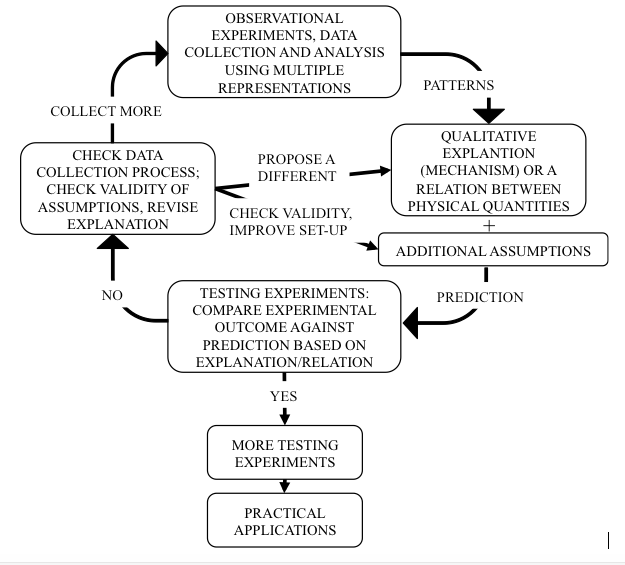
\includegraphics[width=0.7\textwidth]{force-motion-1/islegraphic.png}
	\caption{A model of the process some scientists go through to create knowledge.\cite{etkina_millikan_2015}}\label{me:fig:isle}
\end{figure}

\section{Team roles}

\textbf{Decide on roles} for each group member. The available roles are:

\begin{itemize}
	\item Facilitator: ensures time and group focus are efficiently used
	\item Scribe: ensures work is recorded
	\item Technician: oversees apparatus assembly, usage
	\item Skeptic: ensures group is questioning itself
\end{itemize}

these roles can (will?) rotate each lab, and you will report at the end of the lab report on how it went for each role. If you have fewer than 4 people in your group, then some members will be holding more than one role.

\section{Observation Experiment: Recording and Representing Motion}\label{fm1:sec:obs}

\textbf{Goal:} Record the motion of an object and represent its motion using a motion diagram.

\begin{steps}
	\item go to \url{https://physics.bu.edu/~duffy/HTML5/motion_diagrams.html}
	
	\item click play, watch Cars 1 and 2 (represented by the top (red) and bottom (blue) big dots) drive forward.
	
	\item notice that every second, a small dot is drawn to show where the car was at that time. this creates a visual record of the car's motion.
	
	\item How would you classify the object’s motion: motion with constant rate, increasing rate, decreasing rate? Explain how you decided.
	
	\item increase velocity of second car by dragging the velocity slider to the right.
	
	\item record how the motion diagram changes.
	
	\item imagine that you were given this plot without any velocity information - just the small dots. How could you tell which car was faster? Describe the procedure you would use to determine this.

	\item Observe the motion diagram captured in Figure\ \ref{fm1:fig:slowing}, specifically Car 2. How would you classify the object’s motion: motion with constant rate, increasing rate, decreasing rate? Explain how you decided.
	
%	\item Write a procedure to calculate how 
\end{steps}

\begin{figure}
	\centering
	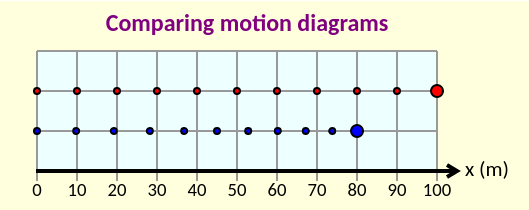
\includegraphics[width=0.6\textwidth]{force-motion-1/motion-diagrams-slowing.png}
	\caption{Motion diagrams of Car 1 (red, top) and Car 2 (blue, bottom). The small dots were marked every 1 second during the cars' motions.}\label{fm1:fig:slowing}
\end{figure}

%\begin{figure}
%	\centering
%	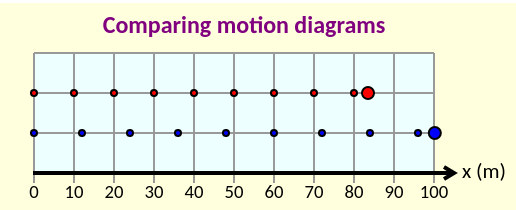
\includegraphics[width=0.5\textwidth]{force-motion-1/motion-diagrams.png}
%	\caption{Motion diagrams of Car 1 (red, top) and Car 2 (blue, bottom). The small dots were marked every 1 second during the cars' motions.}
%\end{figure}

\section{Observation Experiment: Forces Exerted on an Object by	Other Objects}

\textbf{Goal:} Learn to represent forces exerted on an object by other objects in a clear and efficient way.

\textbf{Available Equipment:} Two household objects of different weights and similar shapes, for example a bowling ball and a tennis ball.

Pick up a tennis ball and hold it stationary in your hand. Then pick up a bowling ball and hold it the same way. Do you feel any difference? Now we will learn to represent this difference graphically using force diagrams (sometimes called free-body diagrams).

\textbf{For each situation (tennis ball and bowling ball) do the following:}
\begin{steps}
	\item List all the objects that interact with the ball.  The ball is called the "object of interest" since that's what we are focusing our attention on.  To interact with the ball, most other objects need to be in physical contact with it (the Earth is an exception --- it can interact gravitationally from a distance).
	%Explain how you can represent these interactions on a diagram so that Alex can understand them.
	
	\item Represent the ball with a dot and use an arrow to represent each interaction of another object with the ball. Connect the tails of the arrows to the dot. Label each force arrow with an $\vec{F}$ that has two subscripts. The first subscript represents the object that exerts the force on the object of interest; the second subscript represents the object of interest itself. For example, the force that the hand exerts on the ball can be written as $\vec{F}_{H \rightarrow B}$. Pay attention to the lengths of the arrows on each force diagram.  Should any of them be longer or shorter than others?
	
	\item Indicate what forces "cancel" or "balance" each other. Indicate if there is an "unbalanced" force. Explain how your force diagram is a better way of describing the forces being exerted on an object than written words.
	
	\item Why are forces represented by arrows and not just by numbers or lines?
	
	\item You can compare your force diagram to the one found at \url{https://physics.bu.edu/~duffy/HTML5/force_motion_1D.html} . Notice how the diagram changes when you change the mass.
\end{steps}

\section{Testing Experiment: Does an object’s motion always	occur in the direction of the unbalanced force exerted on it by other objects?}

\textbf{Goal:} Test two ideas (also called \textit{hypotheses}):
\begin{enumerate}[label=(\alph*)]
	\item An object always moves in the direction of the unbalanced force exerted on it by other objects.
	\item An object always changes its motion in the direction of the unbalanced force exerted on it by other objects.
\end{enumerate}

\textbf{Available equipment:} Everything around you. You might be helped by things that roll, and forming a ramp with books. Also the following simulation: \url{https://phet.colorado.edu/sims/html/forces-and-motion-basics/latest/forces-and-motion-basics_en.html} (try the Motion screen in particular)

\begin{framed}
	\textbf{Self-assessment:} To help you improve your scientific abilities, we provide you with self-assessment rubrics.
	A rubric is a method of aligning expectations for performance.
	Self-assessment is determining how well you performed a particular task.
	So, these self-assessment rubrics are designed to help you evaluate your performance while you are designing and performing your experiment.
	
	The complete set of rubrics is available in Appendix~\ref{cha:rubrics}.
		In each lab, your report will be assessed using Rubric F, found in Table~\ref{rubric:f}, as well as 5 additional rubric rows listed in that lab.
		Each week, read through these and use them to evaluate your work as you design and perform the experiment.
		Your instructor will use the same rubrics to determine part of your grade for the lab. In particular, each row will be worth 3 possible points (from ``Missing'' being 0 points to ``Adequate'' being 3 points).
\end{framed}

\textbf{Rubrics to focus on during this experiment:} C1, C2, C4, C7, C8. See Table~\ref{rubric:c} for details.

\begin{steps}
	\item First, think about the two competing ideas that you are testing. Think about how you can use the available equipment to design experiments relevant to both of them. Also, think what the words "test an idea" mean in real life. Does "testing" mean trying to support an idea or trying to disprove an idea? Which approach do you think is more productive? When you come up with at least 2 possible experiments, \textbf{contact an instructor or TA} and discuss your experiments with them.
	
	\item After your discussion with the TA, record the two experiments you are going to perform. Draw pictures and force diagrams for each situation.
	
	\item Make a prediction of the outcome of each experiment if idea (a) were correct.
	
	\item Make a prediction of the outcome of each experiment if idea (b) were correct.
	
	\item Make a table to record the following information for the object: (1) the direction of the motion, (2) the direction of the change in motion, and (3) the direction of the unbalanced force.
	
	\item Perform each experiment and record the outcome in the table.
	
	\item Decide if any of the predictions are consistent with the outcomes of the experiments.
	
	\item Make a judgment about each idea.  That is, decide which, if any, of the ideas are consistent with the outcome of the experiment. Remember, the goal of a testing experiment is to \textbf{disprove} ideas, not to support them.
	
	\item Include arguments for why your judgments are reasonable in your report.
	
	\item The experiment in Section \ref{fm1:sec:obs} was called an observational experiment, and the experiment in this section was called a testing experiment. How do these names reflect the differences in performing these two kinds of experiments? (What aspects does one kind have that the other type does not?)
	
	\item Design, describe, and (if possible) perform two more experiments in which the object does not move in the direction of the unbalanced force. Draw a motion diagram and a force diagram for each experiment.
	
	\item You have represented motion and forces in different ways.  Explain how these representations helped you to find a pattern/relationship between motion and forces.
\end{steps}

\section{Why Did We Do This Lab?}

\begin{steps}
	\item In a paragraph, summarize what you have learned during this first lab in terms of physics content and in terms of the purpose of the two kinds of experiments you designed and performed.
	
	\item Describe how your understanding of the relationship between force and motion is different from your understanding before.
\end{steps}

\section{Group dynamics}

\begin{steps}
	\item Write a 100--200 word reflection on group dynamics and feedback on the lab manual. Address the following topics: who did what in the lab, how did you work together, what successes and challenges in group functioning did you have, and what would you keep and change about the lab write-up?
	
	\item Write a paragraph reporting back from each of the four roles: facilitator, scribe, technician, skeptic. Where did you see each function happening during this lab, and where did you see gaps?
\end{steps}

\section{Report checklist and grading}

The lab grade consists of 3 points for each of seven scientific ability rubric rows (the 5 listed above, which apply just to that section, as well as F1 and F2, applied to the entire report), and 9 points for providing evidence in the lab report of completing all steps of the lab, including answering every question, for a total of 30 points.